% Title: gl2ps_renderer figure
% Creator: GL2PS 1.4.0, (C) 1999-2017 C. Geuzaine
% For: Octave
% CreationDate: Tue Oct 26 19:56:14 2021
\setlength{\unitlength}{1pt}
\begin{picture}(0,0)
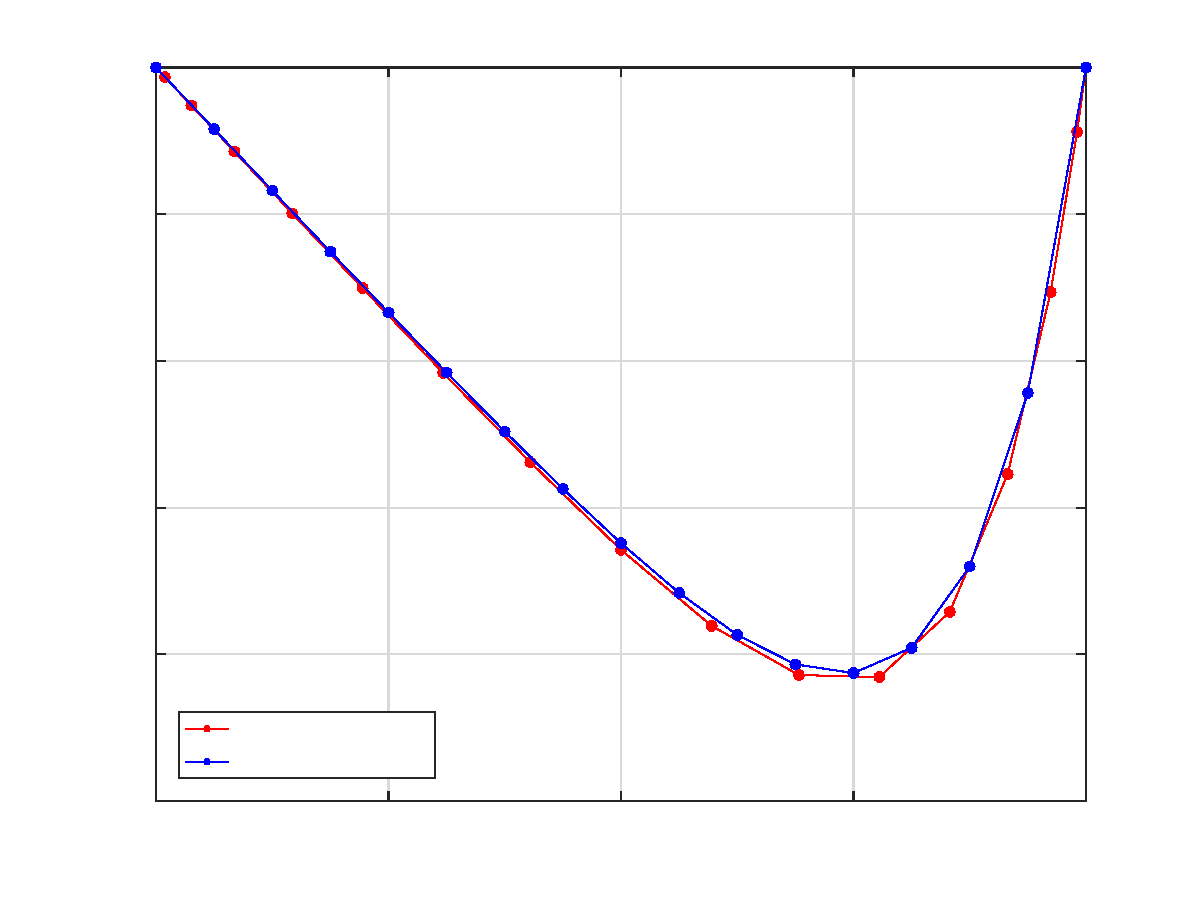
\includegraphics{figures/chap27/OUT/CollVsFD16-inc}
\end{picture}%
\begin{picture}(576,432)(0,0)
\fontsize{10}{0}
\selectfont\put(74.88,40.0183){\makebox(0,0)[t]{\textcolor[rgb]{0.15,0.15,0.15}{{-1}}}}
\fontsize{10}{0}
\selectfont\put(186.48,40.0183){\makebox(0,0)[t]{\textcolor[rgb]{0.15,0.15,0.15}{{-0.5}}}}
\fontsize{10}{0}
\selectfont\put(298.08,40.0183){\makebox(0,0)[t]{\textcolor[rgb]{0.15,0.15,0.15}{{0}}}}
\fontsize{10}{0}
\selectfont\put(409.68,40.0183){\makebox(0,0)[t]{\textcolor[rgb]{0.15,0.15,0.15}{{0.5}}}}
\fontsize{10}{0}
\selectfont\put(521.28,40.0183){\makebox(0,0)[t]{\textcolor[rgb]{0.15,0.15,0.15}{{1}}}}
\fontsize{10}{0}
\selectfont\put(69.8755,47.52){\makebox(0,0)[r]{\textcolor[rgb]{0.15,0.15,0.15}{{-2.5}}}}
\fontsize{10}{0}
\selectfont\put(69.8755,117.936){\makebox(0,0)[r]{\textcolor[rgb]{0.15,0.15,0.15}{{-2}}}}
\fontsize{10}{0}
\selectfont\put(69.8755,188.352){\makebox(0,0)[r]{\textcolor[rgb]{0.15,0.15,0.15}{{-1.5}}}}
\fontsize{10}{0}
\selectfont\put(69.8755,258.768){\makebox(0,0)[r]{\textcolor[rgb]{0.15,0.15,0.15}{{-1}}}}
\fontsize{10}{0}
\selectfont\put(69.8755,329.184){\makebox(0,0)[r]{\textcolor[rgb]{0.15,0.15,0.15}{{-0.5}}}}
\fontsize{10}{0}
\selectfont\put(69.8755,399.6){\makebox(0,0)[r]{\textcolor[rgb]{0.15,0.15,0.15}{{0}}}}
\fontsize{11}{0}
\selectfont\put(298.08,27.0183){\makebox(0,0)[t]{\textcolor[rgb]{0.15,0.15,0.15}{{$x$}}}}
\fontsize{11}{0}
\selectfont\put(298.08,409.6){\makebox(0,0)[b]{\textcolor[rgb]{0,0,0}{{Chebyshev Collocation and Finite Difference Approximations: $N =$ 16}}}}
\fontsize{12}{0}
\selectfont\put(253.44,329.184){\makebox(0,0)[l]{\textcolor[rgb]{0,0,0}{{max collocation error       = 1.928e-11}}}}
\fontsize{12}{0}
\selectfont\put(253.44,301.018){\makebox(0,0)[l]{\textcolor[rgb]{0,0,0}{{max finite difference error = 3.380e-02}}}}
\fontsize{9}{0}
\selectfont\put(112.873,82.1738){\makebox(0,0)[l]{\textcolor[rgb]{0,0,0}{{Chebyshev Collocation}}}}
\fontsize{9}{0}
\selectfont\put(112.873,66.3952){\makebox(0,0)[l]{\textcolor[rgb]{0,0,0}{{Finite Difference}}}}
\end{picture}
